\documentclass[sigconf]{acmart}
\usepackage{listings}
\usepackage{booktabs} % For formal tables

\lstset{language=R,
    basicstyle=\small\ttfamily,
    stringstyle=\color{green},
    morekeywords={TRUE,FALSE},
    deletekeywords={data,frame,length,as,character},
    keywordstyle=\color{blue},
    commentstyle=\color{green},
}

\acmArticle{4}
\acmPrice{15.00}

\begin{document}
\title{ISyE 6416 Homework 1: Regression in R}
\subtitle{Linear regression analysis and model selection}

\author{Shixiang Zhu}
\affiliation{
  \institution{Georgia Institute of Technology}
  \city{Atlanta}
  \state{Georgia}
}
\email{shixiang.zhu@gatech.edu}

\begin{abstract}
For this analysis, the aim of linear regression is to model the relationship between three auto manufacturers: Toyata Motor Corp., Ford Motor Corp., and GM. Treat the log returns of GM as response and log returns of Toyota and Ford as predictors. We fit a linear regression model in R and perform necessary model diagnostics. By analyzing the given dataset, we draw the conclusion on whether linear regression is a useful tool for this dataset and find out which predicotrs are playing important roles in this relationship.
\end{abstract}

\keywords{linear regression, model selection, log returns}

\maketitle
\newcommand{\norm}[1]{\left\lVert#1\right\rVert}
\section{Introduction}

In this report, we build a linear regression model for the given dataset to help a banker use the log returns of Toyota and Ford to interpret the log returns of GM. First we evaluate the statistical significance for 
Linear regression is used to predict the value of an outcome variable (response) based on one or more input variables (predictor). The goal of linear regression model is to establish a linear relationship between predictors and responses. 

\section{Problem Formulation}

The aim of linear regression is to model the log returns of GM. $Y$ as a function of the log returns of Toyota $X_1$ and the log returns of Ford $X_2$. The function of their relationship can be defined as follows:
$$Y = \beta_0 + \beta_1 X_1 + \beta_2 X_2 + \epsilon$$
where $\beta_0$ is the intercept and $\beta_1$, $\beta_2$ are the regression coefficients of $X_1$, $X_2$ respectively. $\epsilon$ is the error term.

By definition of linear regression, the objective function for this problem is:

$$\min_{\beta} \norm{ Y - X \beta }^2_2 \iff \min_{\beta_0, \beta_1, \beta_2} \sum_{i=1}^{n} {(y_i - \beta_0 - \beta_1 x_{i1} - \beta_2 x_{i2})^2}$$


\section{Model Estimation}

A large number of procedures have been developed for parameter estimation inference in linear regression. Those methods are different in some aspects like computational simplicity, presence of a closed-form solution, robustness with respect to heavy-tailed distributions, etc. In this report, we apply the simplest and thus most common estimator to our linear regression model, ordinary least squares (OLS), which is the exact way how we estimate parameters in R. 

The OLS method minimizes the sum of squared residuals, and leads to a closed-form expression for the estimated value of the unknown parameter $\beta$:

$$\hat{\beta} = (\mathbf{X}^\top \mathbf{X})^{-1} \mathbf{X}^\top \mathbf{Y} = (\sum{\mathbf{x}_i\mathbf{x}_i^\top})^{-1} (\sum{\mathbf{x}_i} y_i) $$ 

In addition, the OLS estimaor is also identical to the maximum likelihood estimator (MLE) under the normality assumption for the error terms \cite{test} (i.e. if the errors are i.i.d normal distribution $\mathcal{N}(0, \sigma^2)$.) 

% in the Bibliography section of your
% article will occur throughout the text of your article.
% You should use BibTeX to automatically produce this bibliography;
% you simply need to insert one of several citation commands with
% a key of the item cited in the proper location in
% the \texttt{.tex} file~\cite{Lamport:LaTeX}.
% The key is a short reference you invent to uniquely
% identify each work; in this sample document, the key is
% the first author's surname and a
% word from the title.  This identifying key is included
% with each item in the \texttt{.bib} file for your article.

% Immediately following this sentence is the point at which
% Table~\ref{tab:freq} is included in the input file; compare the
% placement of the table here with the table in the printed
% output of this document.

% \begin{table}
%   \caption{Frequency of Special Characters}
%   \label{tab:freq}
%   \begin{tabular}{ccl}
%     \toprule
%     Non-English or Math&Frequency&Comments\\
%     \midrule
%     \O & 1 in 1,000& For Swedish names\\
%     $\pi$ & 1 in 5& Common in math\\
%     \$ & 4 in 5 & Used in business\\
%     $\Psi^2_1$ & 1 in 40,000& Unexplained usage\\
%   \bottomrule
% \end{tabular}
% \end{table}

% \subsection{Figures}

\begin{figure}
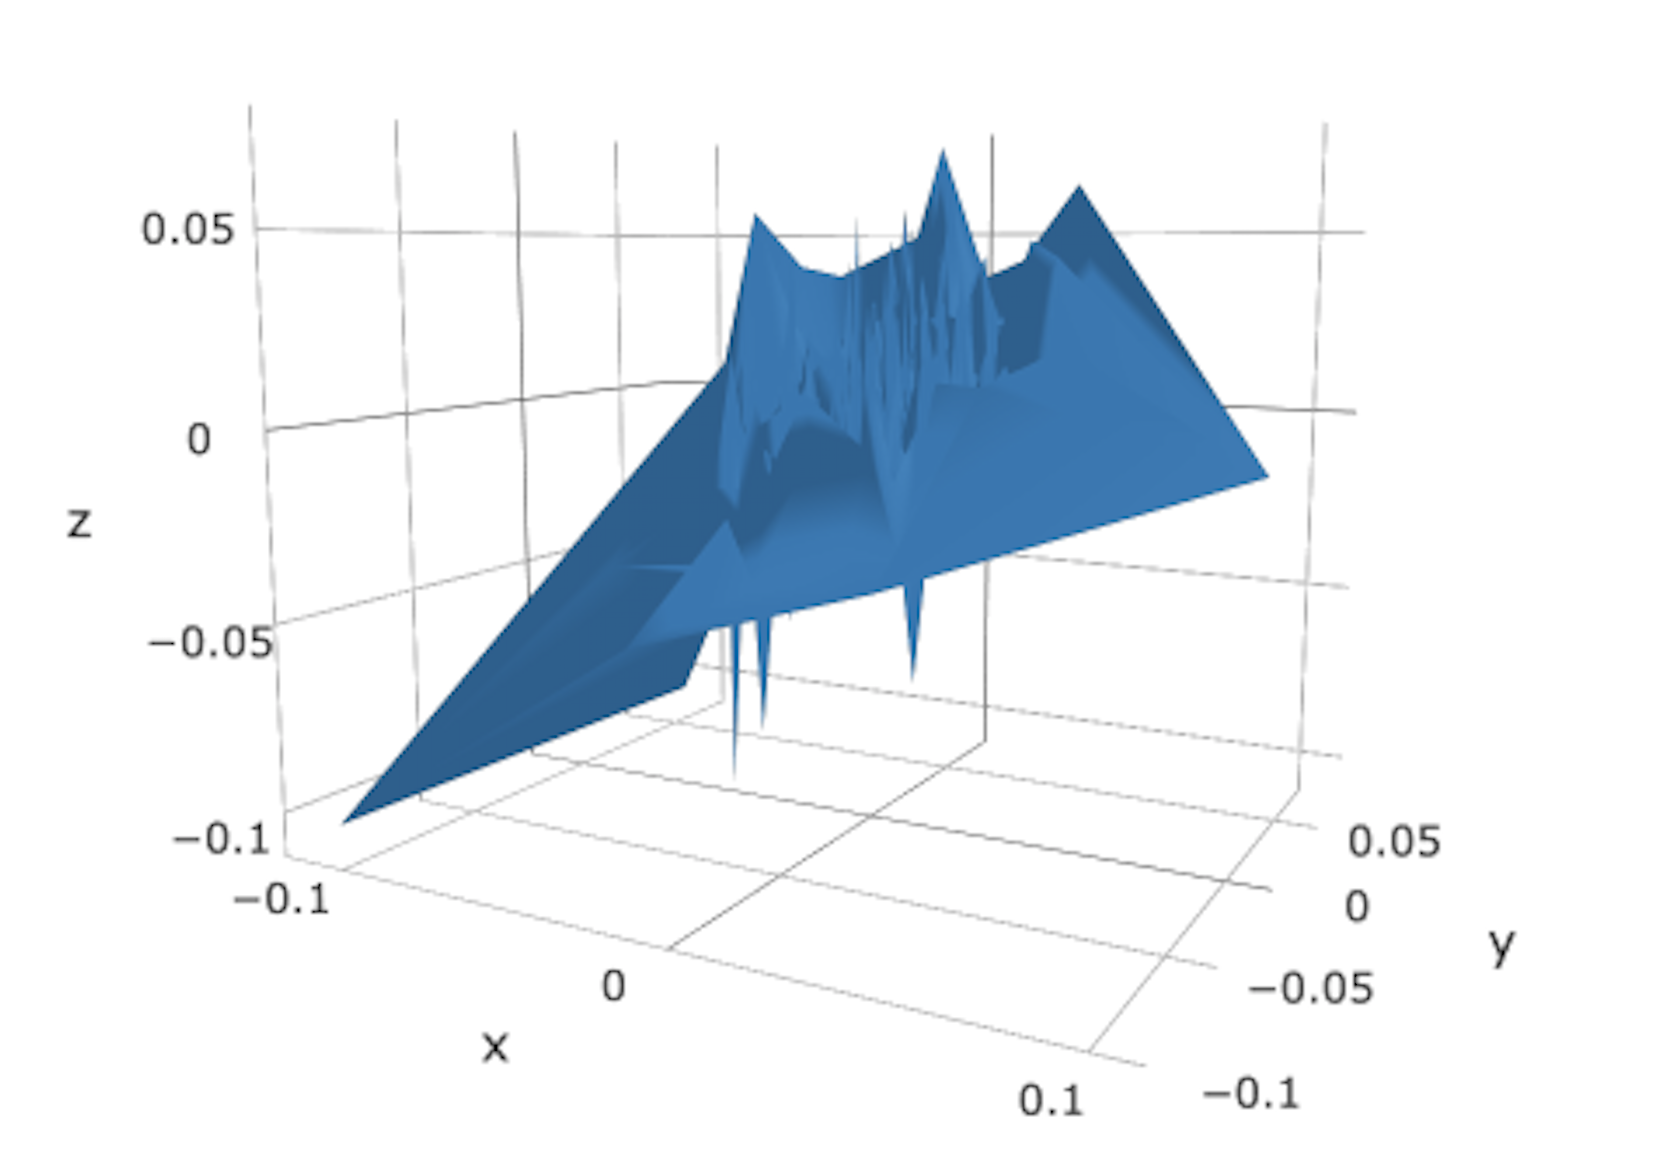
\includegraphics[scale=0.3]{surface}
\caption{Surface of GM. vs. Toyota Motor Corp. and Ford Motor Corp.}
\label{img:surface}
\end{figure}

\begin{table}[]
\centering
\caption{Summary of raw data}
\label{tab:rawdata}
\begin{tabular}{l|lll}
        & \textbf{Toyota Motor Corp.} & \textbf{Ford Motor Corp.} & \textbf{GM.}        \\ \hline
Min.    & -0.1132272                  & -9.481e-02                & \textit{-0.1061545} \\
1st Qu. & -0.0084958                  & -9.368e-03                & \textit{-0.0119514} \\
Median  & 0.0005180                   & -2.082e-04                & \textit{0.0004089}  \\
Mean    & 0.0008693                   & 7.535e-05                 & \textit{0.0001701}  \\
3rd Qu. & 0.0105164                   & 1.122e-02                 & 0.0116914           \\
Max.    & 0.1049635                   & 7.429e-02                 & 0.0744415          
\end{tabular}
\end{table}

\begin{table*}[t]
\centering
\caption{Summary of linear regression}
\label{tab:lr}
\begin{tabular}{lllll}
\hline
\multicolumn{5}{l}{\textbf{Residuals}} \\
\textit{Min} & \textit{1Q} & \textit{Median} & \textit{3Q} & \textit{Max} \\
-0.062848 & -0.009649 & -0.000405 & 0.008977 & 0.057515 \\ \hline
\multicolumn{5}{l}{\textbf{Coefficients}} \\
 & \textit{Estimate} & \textit{Std. Error} & \textit{t value} & \textit{Pr(\textgreater|t|)} \\
\textit{(Intercept)} & 7.049e-05 & 5.914e-04 & 0.119 & 0.905 \\
\textit{`Ford Motor Corp.`} & 6.145e-01 & 3.132e-02 & 19.619 & \textless2e-16 \\
\textit{`Toyota Motor Corp.`} & 6.132e-02 & 3.784e-02 & 1.621 & 0.106 \\ \hline
\textbf{Residual standard error} & \multicolumn{4}{l}{0.01572 on 706 degrees of freedom} \\
\textbf{Multiple R-squared} & 0.3775 & \textbf{Adjusted R-squared} & \multicolumn{2}{l}{0.3757} \\
\textbf{F-statistic} & 214.1 on 2 and 706 DF & \textbf{p-value} & \multicolumn{2}{l}{\textless 2.2e-16} \\ \hline
\end{tabular}
\end{table*}

\section{Experiments}

In experiments, we use the dataset provided on class that comes with R. Before building the linear regression model, we start to take a look at the raw dataset first to analyze and understand the variables intuitively. First of all, Surface plot can help visualize the linear relationships between the response variables and predictor variables. Ideally, in linear regression, their relationship can be model as a plane in this space. As shown in Fig. \ref{img:surface}, $x$-axis and $y$-axis mean the log returns of Toyota Motor Corp. and Ford Motor Corp. respectively, $z$-axis is the the log returns of GM. Besides graphical analysis, we can also study their statistical property. As reported in Table~\ref{tab:rawdata}, the log returns of GM. seems to be highly correlated with Toyota. 

\subsection{Linear Regression Diagnostics}

Before actually using linear regression model, we need to ensure it is statistically significant. Since a larger t-value indicates it is less likely that the coefficient is not equal to zero purely by chance and the corresponding p-value would be relatively low, which means the coefficients are significant. As reported in Table~\ref{tab:lr}, the p-value of Ford Motor Corp. is significantly lower than 0.05, we can safely reject the null hypothesis that coefficient $\beta_2$ of the predictor is zero. However, the p-value of Toyota Motor Corp. is slightly larger than 0.05, which means the log returns of Toyota Motor Corp. is not statistically significant to the log returns of GM. As to R-Squared and Adj R-Squared value, they are kind of lower than empirical value 0.70 (actually R-Squared is not a good criterion, since it always increase with the model size).

In additin, we also check the diagnostic plots for further analysis of this regression model, in particular, they show residuals in four different ways: \texttt{1. Normal Q-Q plot}: Fig. \ref{img:qqplot} shows residuals follow a straight line well when residuals lie between -2 to 2, within this range, the residuals perfectly matched normal distribution. \texttt{2. Residuals vs Fitted plot}: 
Fig. \ref{img:rfplot} shows there is no obvious non-linear pattern in residuals, which is a good indication to our linear regression model. \texttt{3. Residuals vs Leverage plot}: Fig. \ref{img:rlplot} is the typical look when there is no influential case, or cases. we can barely see Cook's distance lines (a red dashed line) because all cases are well inside of the Cook's distance lines. \texttt{4. Scale vs Location plot}: as shown in Fig. \ref{img:slplot}, we can tell there is a parabola (the red line) clearly. Residuals are spread inequally along the ranges of predictors, it begins to spread wider along the x-axis as it passes to two end. 

\subsection{Model Selection}

Generally speaking, the linear regression model we built is fairly good in terms of the results of diagnostics. But we can still try to improve it by model selection. As we mentioned above, we can remove the predictor of Toyota Motor Corp. from the model according to their p-values. The rebuilt model shows a minor improvement on BIC and AIC criterion and other statistics, however, on the whole, their performance on prediction or interpolation are essentially the same. We can draw the conclusion that our first linear regression model can be utilized to model the log returns of these three motor companies, and the model can gain a small benefit by removing the predictor of Toyota Motor Corps, but it is not required. 

% \begin{figure}
% \includegraphics[height=1in, width=1in]{fly}
% \caption{A sample black and white graphic
% that has been resized with the \texttt{includegraphics} command.}
% \end{figure}

% \begin{figure*}
% \includegraphics{flies}
% \caption{A sample black and white graphic
% that needs to span two columns of text.}
% \end{figure*}

% \begin{figure}
% \includegraphics[height=1in, width=1in]{rosette}
% \caption{A sample black and white graphic that has
% been resized with the \texttt{includegraphics} command.}
% \end{figure}

% Here is a theorem:
% \begin{theorem}
%   Let $f$ be continuous on $[a,b]$.  If $G$ is
%   an antiderivative for $f$ on $[a,b]$, then
%   \begin{displaymath}
%     \int^b_af(t)\,dt = G(b) - G(a).
%   \end{displaymath}
% \end{theorem}

% Here is a definition:
% \begin{definition}
%   If $z$ is irrational, then by $e^z$ we mean the
%   unique number that has
%   logarithm $z$:
%   \begin{displaymath}
%     \log e^z = z.
%   \end{displaymath}
% \end{definition}

% \begin{proof}
%   Suppose on the contrary there exists a real number $L$ such that
%   \begin{displaymath}
%     \lim_{x\rightarrow\infty} \frac{f(x)}{g(x)} = L.
%   \end{displaymath}
%   Then
%   \begin{displaymath}
%     l=\lim_{x\rightarrow c} f(x)
%     = \lim_{x\rightarrow c}
%     \left[ g{x} \cdot \frac{f(x)}{g(x)} \right ]
%     = \lim_{x\rightarrow c} g(x) \cdot \lim_{x\rightarrow c}
%     \frac{f(x)}{g(x)} = 0\cdot L = 0,
%   \end{displaymath}
%   which contradicts our assumption that $l\neq 0$.
% \end{proof}

\begin{figure}[h!]
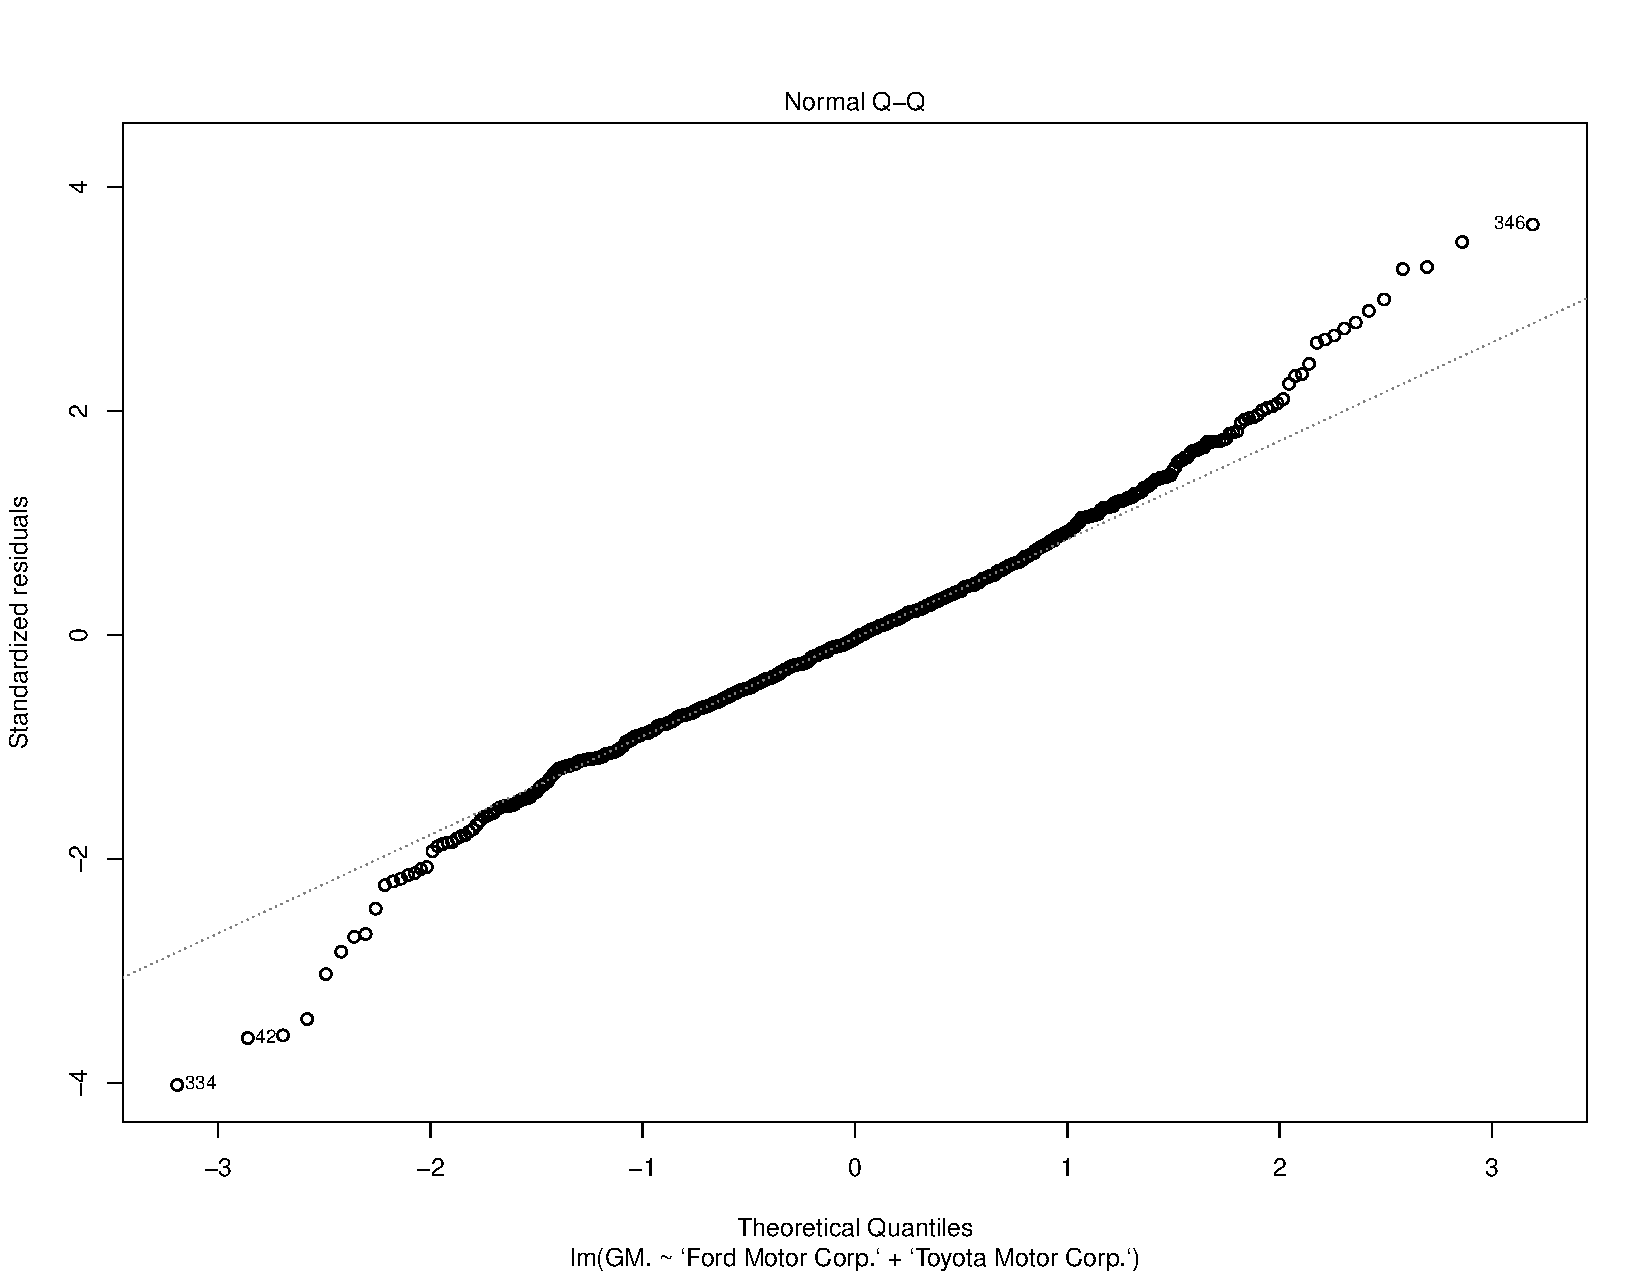
\includegraphics[height=2in, width=2in]{qqplot}
\caption{Normal Q-Q Plot}
\label{img:qqplot}
\end{figure}

\begin{figure}[h!]
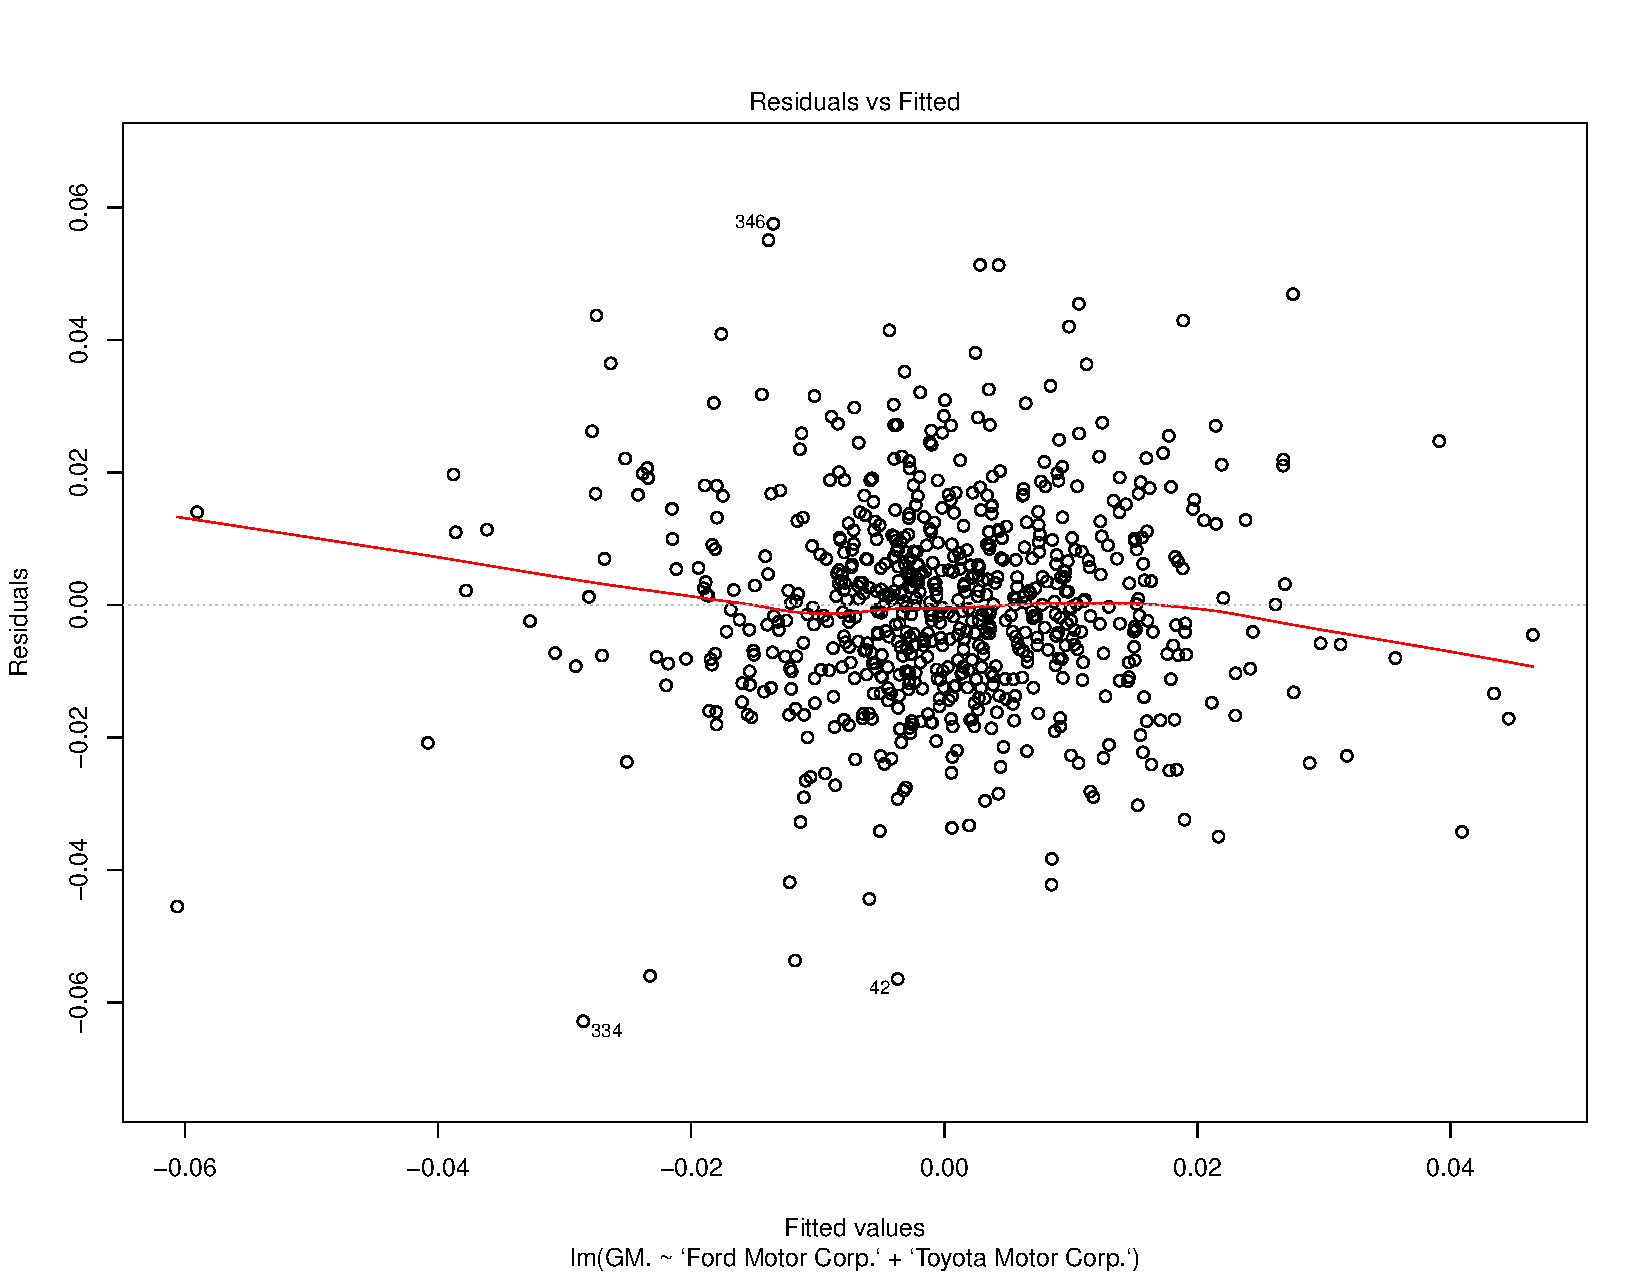
\includegraphics[height=2in, width=2in]{residuals-fitted}
\caption{Residuals-Fitted Plot}
\label{img:rfplot}
\end{figure}

\section{Conclusions}
In this report, we build a linear regression model for three motor companies and briefly analyze the diagnostics of the model. In the basis of the results of the experiments, we reach the conclusion that it is a good model for intercepting the log returns of GM. by using the log returns of Toyota and Ford. We can also remove the predictor of Toyota to improve our model a little bit. 
%\end{document}  % This is where a 'short' article might terminate



\begin{figure}[h!]
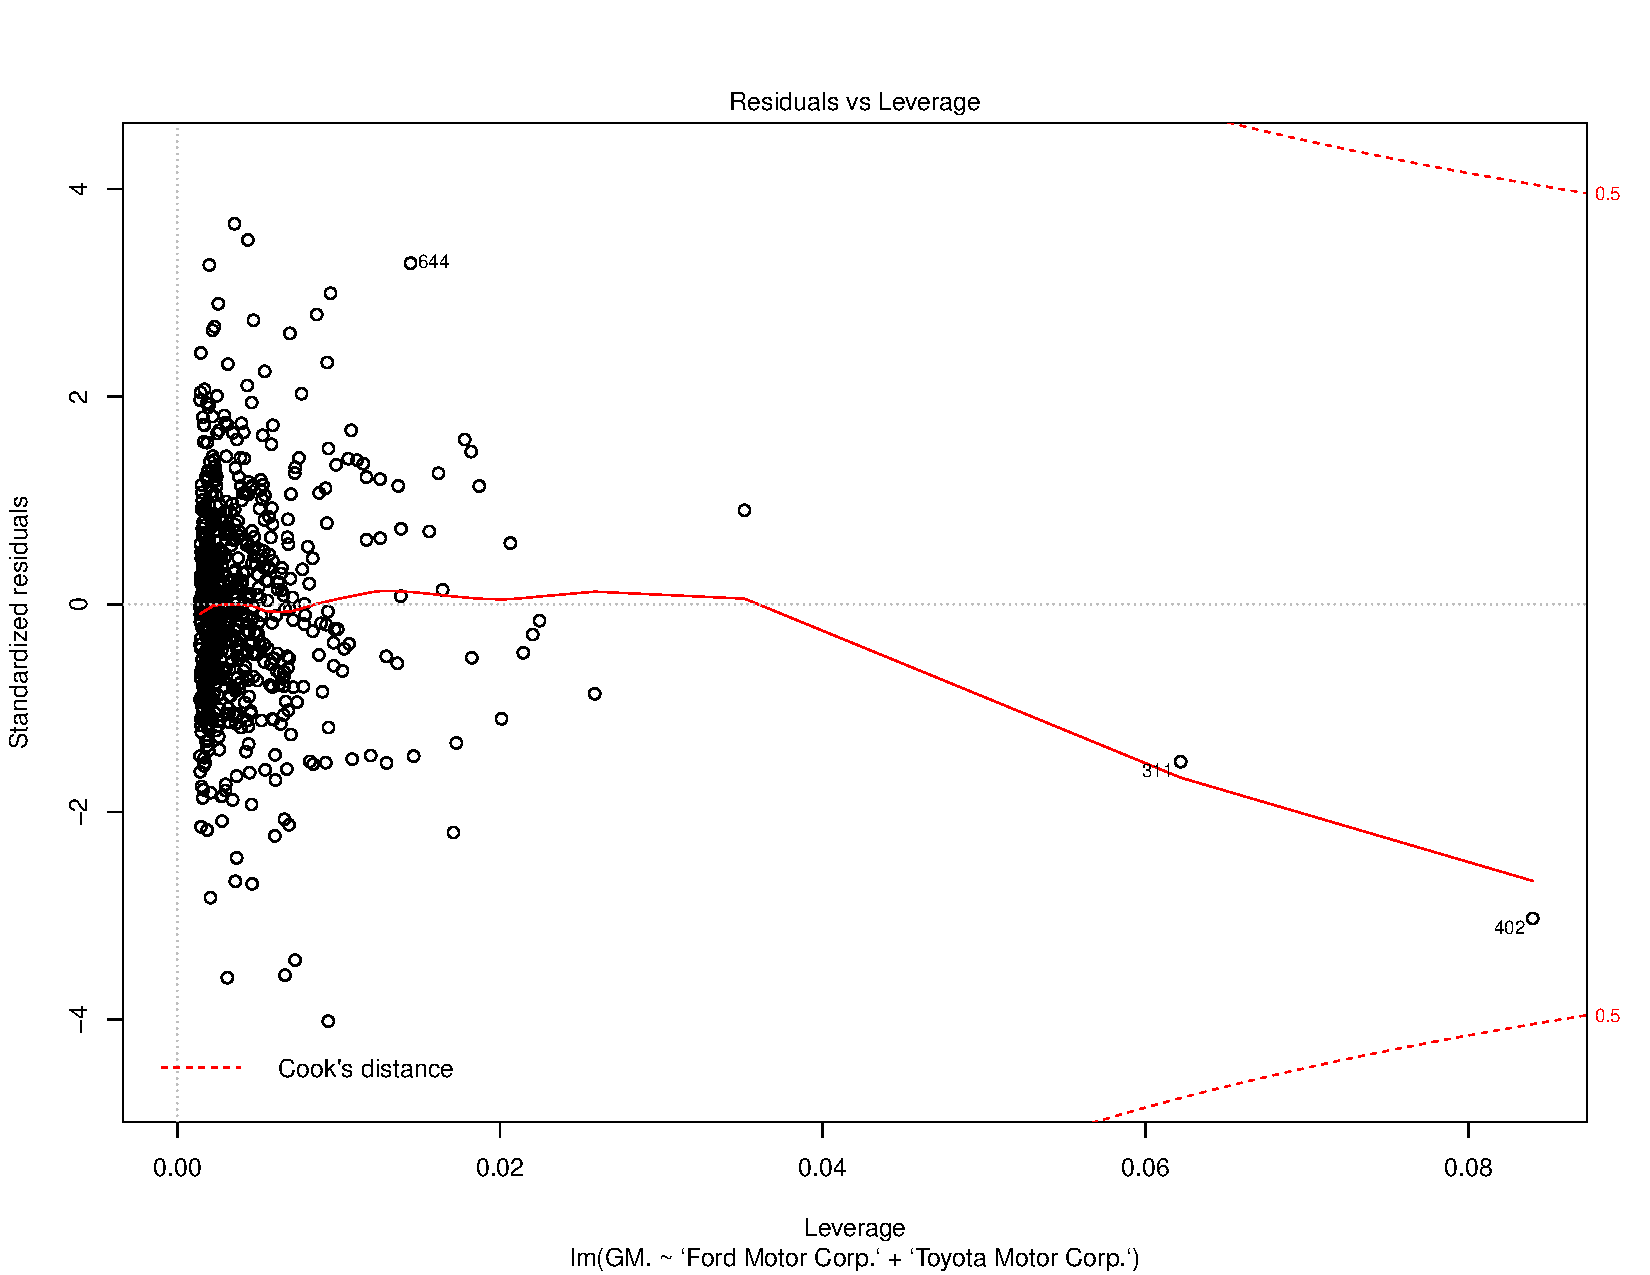
\includegraphics[height=2in, width=2in]{residuals-leverage}
\caption{Residuals-Leverage Plot}
\label{img:rlplot}
\end{figure}

\begin{figure}[h!]
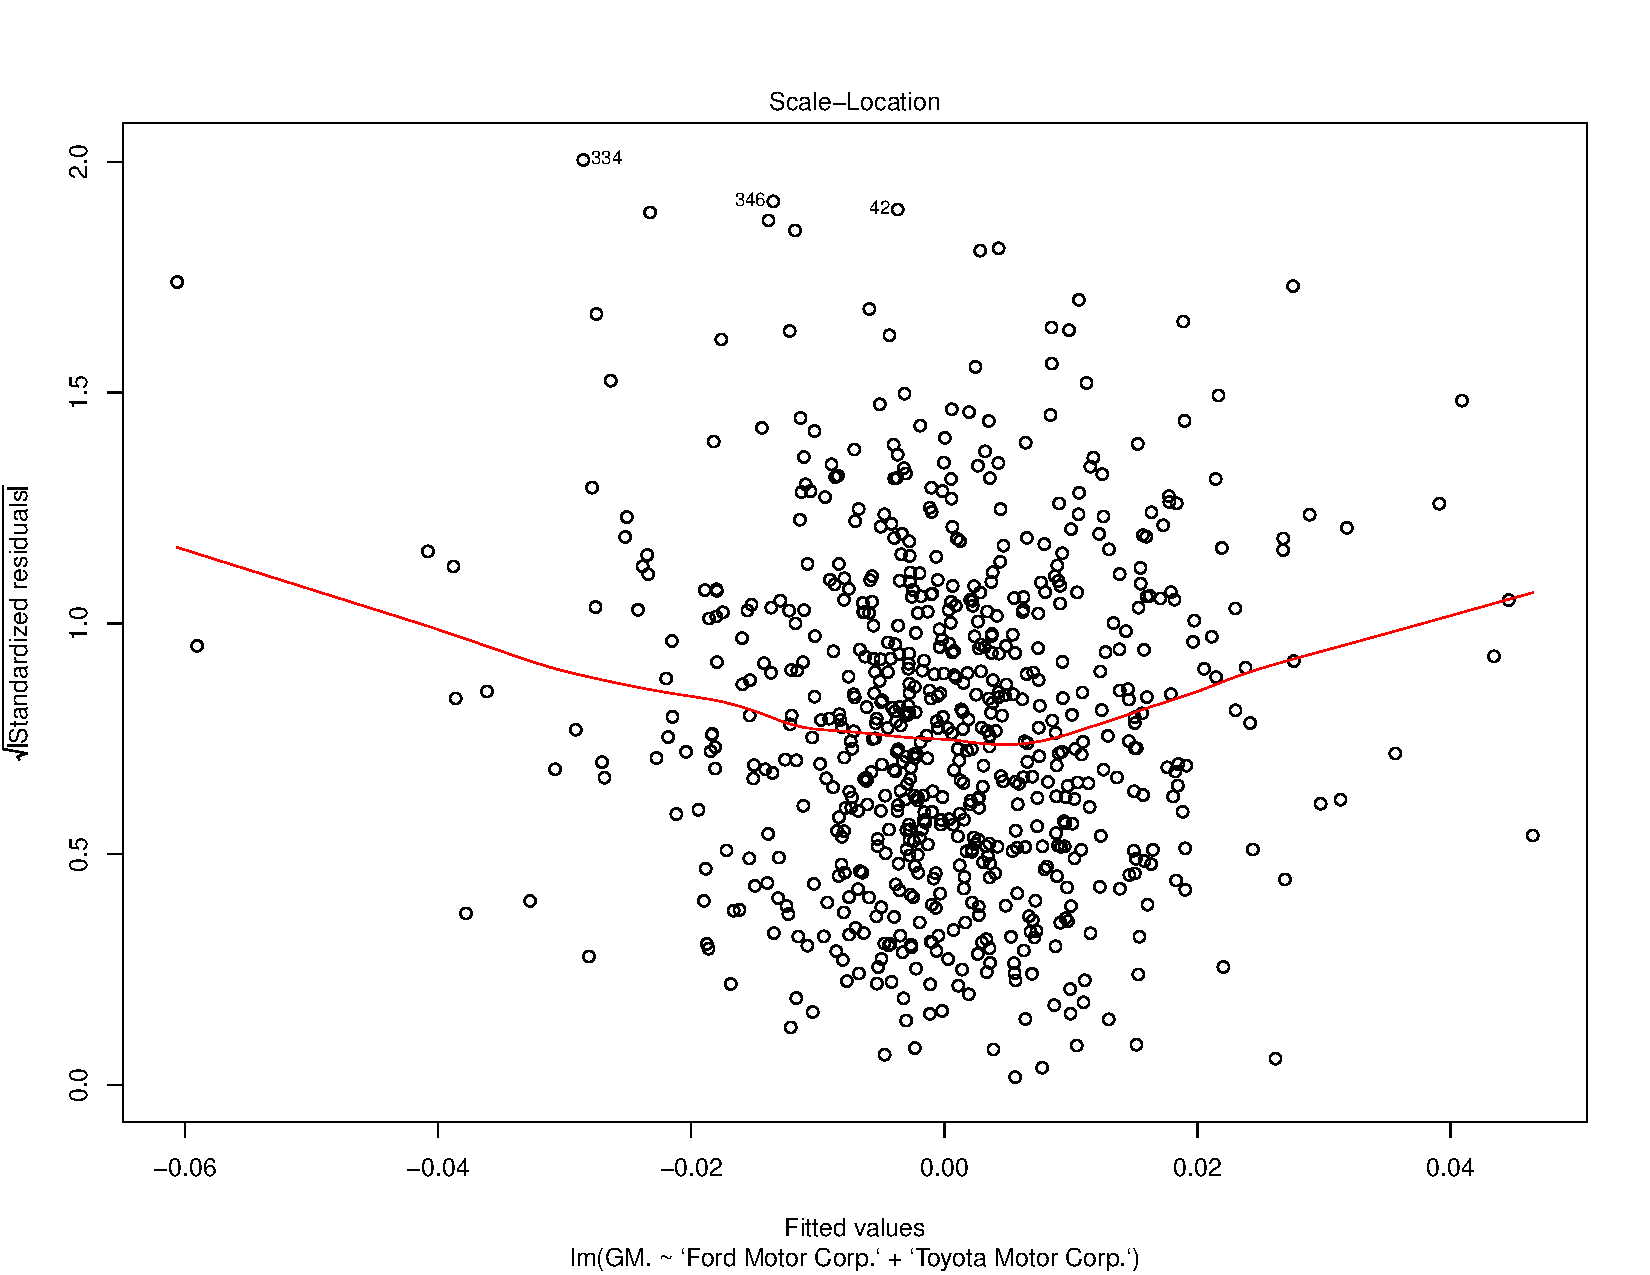
\includegraphics[height=2in, width=2in]{scale-location}
\caption{Scale-Location Plot}
\label{img:slplot}
\end{figure}


% \bibliographystyle{ieeetr}
% \bibliography{refs}

\end{document}
